\section{Performance of OOD detectors calibrated on training ID data}
\label{section:real-classification}

Figure \ref{fig:image-classification} presents the analysis of recognition capabilities for outlierness measures and utilized representation models. The classification of testing samples was performed with respect to the training data – calibrated so that the 95\% of training samples are properly recognized as in-distribution data. Just like in case of AUROC scores, the~obtained scores for each measure differ between representations and no single universal recommendation can be given.

The results show similar observation as made with the numerical simulations (chapter~\ref{chapter:simulations}) for MD – in considered experiment layout (ImageNet as training data), the available number of training samples $n$ was too low for the dimension $d$ of feature space, so the measure's sensitivity was dramatically low. Under the given criteria, i.e., recognition with respect to the training samples, MD spuriously recognizes all in-distribution testing samples as outliers. However, as per figure \ref{fig:image-auroc}, the MD offers satisfying separability between ID and OOD data (i.e., reaching one of the top AUROC scores), at least in cases where it was possible to utilize (except ConvNeXT and ResNet). This suggest a~potential for MD being a~fine OOD detector, although a~practical utilization in such conditions would requite the threshold calibration using validation data – which is still at least questionable recommendation in the context of robustness and safety-critical applications.

An~alternative commonly proposed in literature for such cases is the utilization of MD variant with pooled covariance matrix – MDP. This variant performs surprisingly well in terms of in-distribution samples recognition (sensitivity), while also maintaining satisfying specificity in most of the cases (except EfficientNet and ResNet). Yet, the best outlierness method overall in this task appears to be SED, reaching top scores for both sensitivity and specificity for every representation except for EfficientNet, where the best measure turned out to be kNN.

The result of classification performed on text documents are presented in figure \ref{fig:text-classification} for completeness. The best metric overall appears to be LOF here, competing closely with SED and kNN for BERT representation. Notably the observed scores are higher for classification task on the short text documents (banking77).

Note the accuracy metric is not presented in this chapter, as due to experiment organization (50 ID samples vs thousands of OOD examples) the results would be heavily biased towards the specificity value anyway. Hence, only the sensitivity and specificity metrics are used for comparison.


\begin{figure}[t]
    % StreamLit settings: width=9, height=5
    \centering
    \begin{subfigure}[b]{\textwidth}
        \centering
        \caption{\small Correctly recognized in-distribution samples (ImageNet)}
        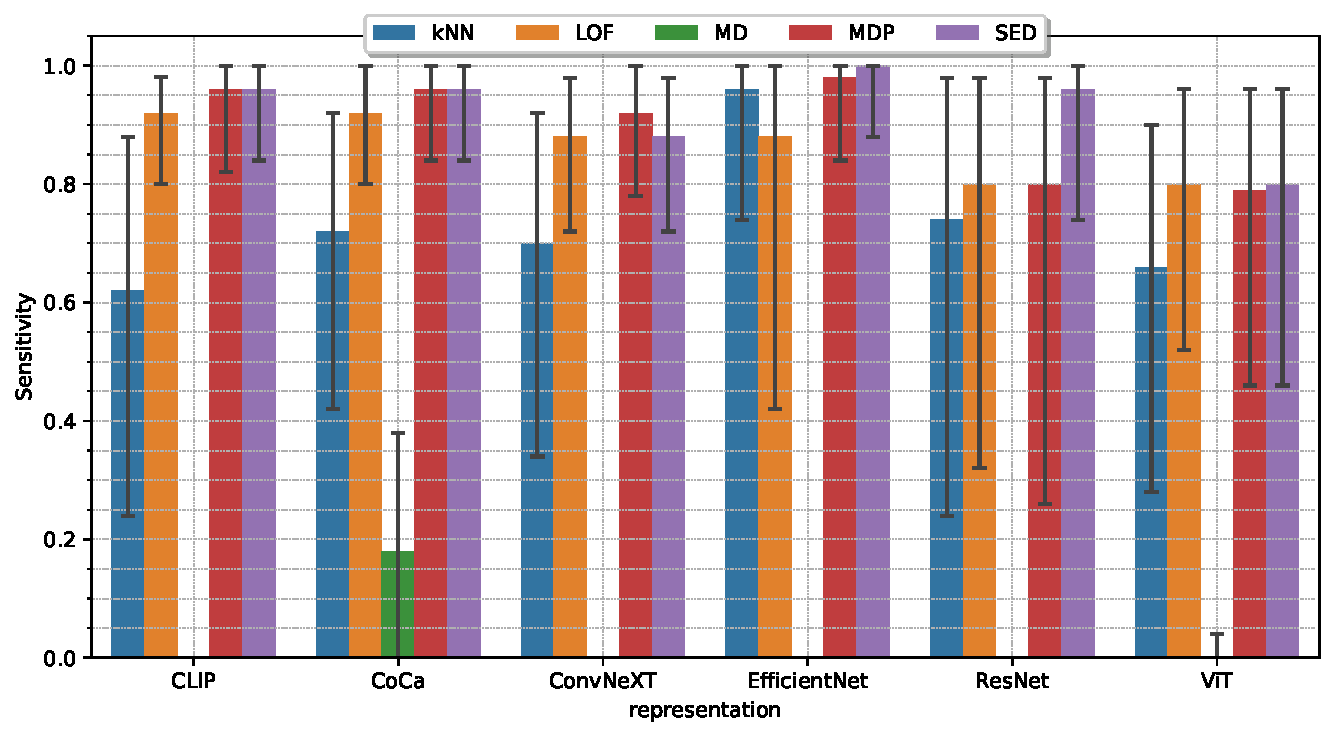
\includegraphics[width=\textwidth]{images/real-classification/barplot-ImageNet-sens_95(representation,model)-representation_CLIP,CoCa,ConvNeXT,EfficientNet,ResNet,ViT-class_0,999-data_ALL.pdf}
        \label{fig:imagenet-sensitivity}
    \end{subfigure}
    \begin{subfigure}[b]{\textwidth}
        \centering
        \caption{\small Correctly recognized out-of-distribution samples (outliers)}
        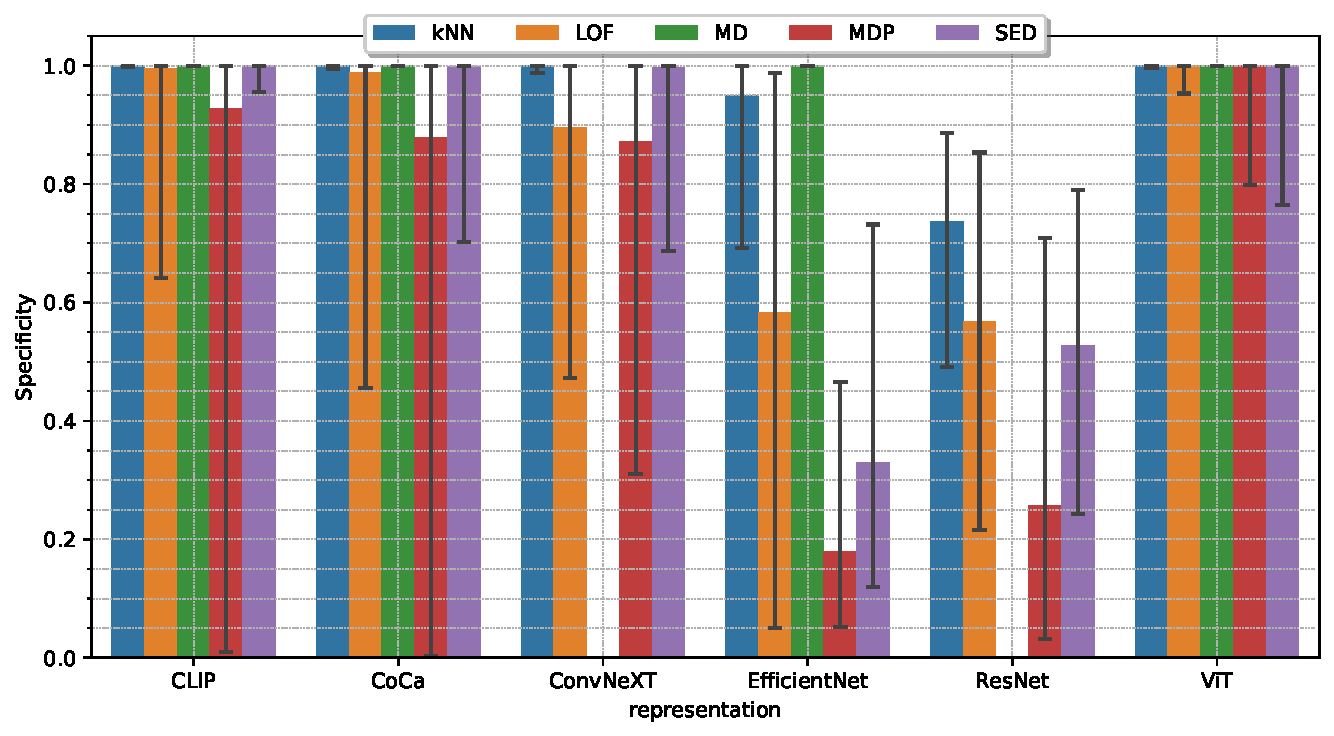
\includegraphics[width=\textwidth]{images/real-classification/barplot-ImageNet-spec_95(representation,model)-representation_CLIP,CoCa,ConvNeXT,EfficientNet,ResNet,ViT-class_0,999-data_ALL.pdf}
        \label{fig:imagenet-specificity}
    \end{subfigure}
    \caption{Results of the image data classification with respect to the training samples. Rejection threshold set so that 95\% of the training data would be correctly recognized as in-distribution. Outliers consist of samples from 7 datasets: ImageNet-O, iNaturalist, NINCO, OpenImage-O, Places365, SUN2012 and Textures.}
    \label{fig:image-classification}
\end{figure}

\begin{figure}[t]
    % StreamLit settings: width=9, height=3
    \centering
    \begin{subfigure}[b]{0.9\textwidth}
        \centering
        \caption{\small Correctly recognized in-distribution samples (20newsgroups)}
        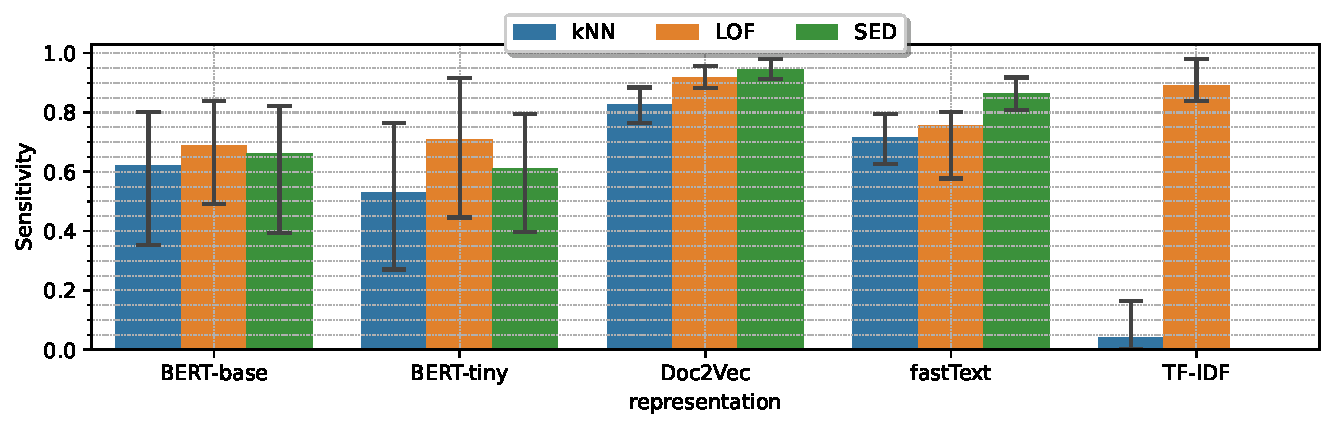
\includegraphics[width=\textwidth]{images/real-classification/barplot-20newsgroups-sens_95(representation,model)-representation_BERT-base,BERT-tiny,Doc2Vec,fastText,TF-IDF-class_0,16-data_outlier.pdf}
        \label{fig:20newsgroups-sensitivity}
    \end{subfigure}

    \vspace{-0.5em}
    \begin{subfigure}[b]{0.9\textwidth}
        \centering
        \caption{\small Correctly recognized out-of-distribution samples (20newsgroups outliers)}
        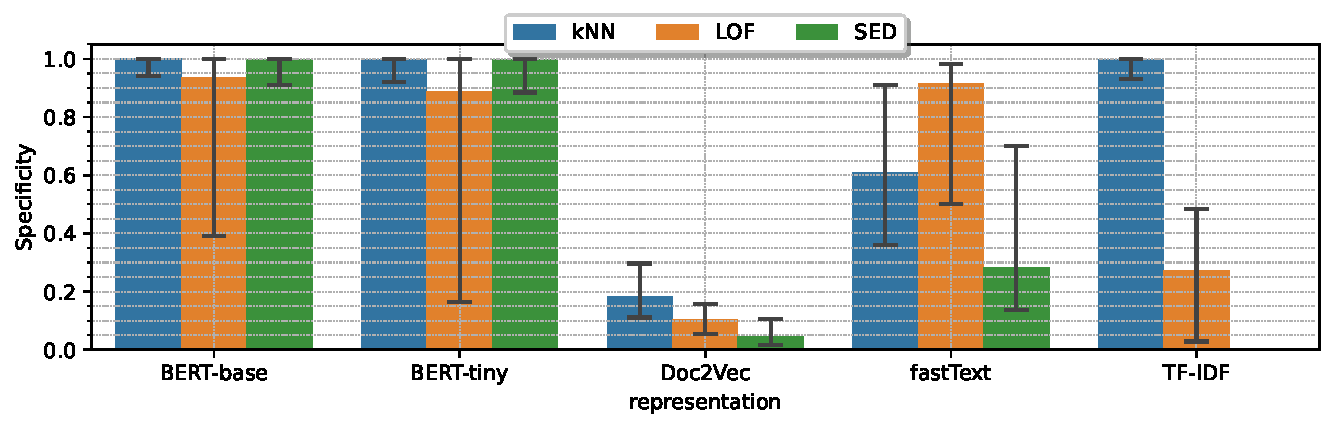
\includegraphics[width=\textwidth]{images/real-classification/barplot-20newsgroups-spec_95(representation,model)-representation_BERT-base,BERT-tiny,Doc2Vec,fastText,TF-IDF-class_0,16-data_outlier.pdf}
        \label{fig:20newsgroups-specificity}
    \end{subfigure}

    \begin{subfigure}[b]{0.9\textwidth}
        \centering
        \caption{\small Correctly recognized in-distribution samples (banking77)}
        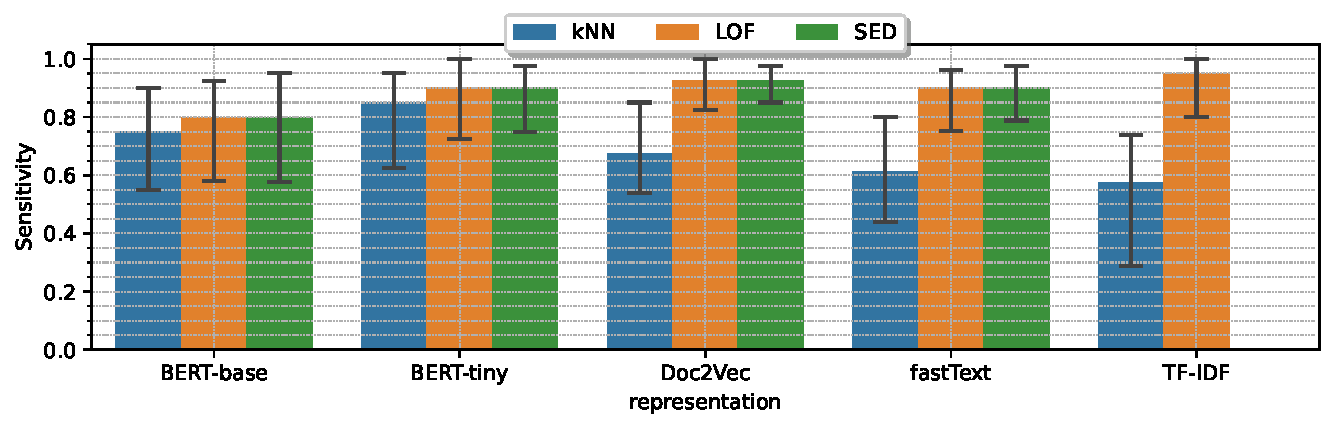
\includegraphics[width=\textwidth]{images/real-classification/barplot-banking77-sens_95(representation,model)-representation_BERT-base,BERT-tiny,Doc2Vec,fastText,TF-IDF-class_0,61-data_outlier.pdf}
        \label{fig:banking77-sensitivity}
    \end{subfigure}

    \vspace{-0.5em}
    \begin{subfigure}[b]{0.9\textwidth}
        \centering
        \caption{\small Correctly recognized out-of-distribution samples (banking77 outliers)}
        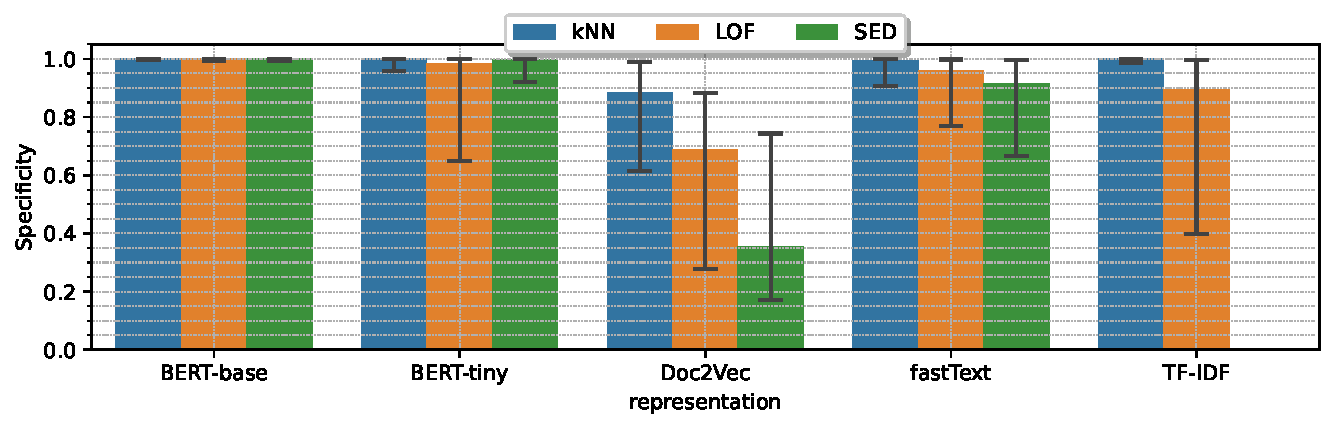
\includegraphics[width=\textwidth]{images/real-classification/barplot-banking77-spec_95(representation,model)-representation_BERT-base,BERT-tiny,Doc2Vec,fastText,TF-IDF-class_0,61-data_outlier.pdf}
        \label{fig:banking77-specificity}
    \end{subfigure}

    \caption{The classification of text documents with respect to the training datasets. Rejection threshold set at $TPR = 95\%$ of the scores obtained for training data.}
    \label{fig:text-classification}
    \vspace{-1.5em}
\end{figure}

\cleardoublepage{}
